% === Revised Section 3: Prediction = Compression ===
%
% This file is a drop-in replacement for lines 309--445 of
% prediction_compression_intelligence_notes.tex.  It assumes the
% preamble already loads tcolorbox (with [most] and the breakable+skins
% libraries), amsmath, amssymb, tikz, hyperref, cleveref, and defines
% the {intuition} tcolorbox.  The additions below are the only new
% preamble pieces required.

% ---------------------------------------------------------------------------
% NEW PREAMBLE ADDITIONS NEEDED (add once, near the existing \newtcolorbox):
% ---------------------------------------------------------------------------
%
% \usepackage{tikz}
% \usetikzlibrary{positioning}
% \usepackage{listings}
% \lstset{basicstyle=\ttfamily\small, breaklines=true, columns=fullflexible}
%
% \newtcolorbox{activity}[1][]{
%   breakable, enhanced,
%   colback=blue!5, colframe=blue!55!black,
%   coltitle=white, fonttitle=\bfseries,
%   title={Activity},
%   boxrule=0.6pt,
%   left=6pt,right=6pt,top=4pt,bottom=4pt,
%   #1
% }
%
% \newtcolorbox{decisionbox}[1][]{
%   breakable, enhanced,
%   colback=green!5, colframe=green!45!black,
%   coltitle=white, fonttitle=\bfseries,
%   title={For the decision-maker},
%   boxrule=0.6pt,
%   left=6pt,right=6pt,top=4pt,bottom=4pt,
%   #1
% }
% ---------------------------------------------------------------------------


\section{Prediction \texorpdfstring{$\Leftrightarrow$}{<=>} Compression
         (Shannon's half of the bridge)}
\label{sec:pred-comp}

\begin{intuition}
A predictor that assigns probabilities to the next word is, mechanically,
a compressor; its error rate and its compression rate are the same
number wearing different clothes (see \cref{thm:ce-code} and
\cref{cor:ppl}).

\medskip
\textbf{The two-consultants analogy (postage version).}  Two
consultants write up the same quarter.  Both are earnest.  The one
who understands your business writes a one-pager: \emph{revenue up
$4\%$, driven by Zurich, offset by FX.}  The one whose mental model
is slightly off writes ten pages of hedging --- because every
surprise in the data costs her extra sentences.  Both describe
reality perfectly; only one \emph{compresses} it.

Think of it as postage.  The true entropy $H(p)$ is the postage a
perfectly-informed sender pays.  Cross-entropy $H(p,q)$ is the
postage you actually pay when your delivery model is $q$ but the
world is $p$.  The difference, $H(p,q) - H(p)$, is the
\textbf{surcharge for being wrong}, and information theory has a
name for it: the Kullback--Leibler divergence $D_{\mathrm{KL}}(p\|q)$.

\medskip
\textbf{A concrete, addable number.}  Suppose tomorrow's stock move
is \emph{up} with probability $0.9$ and \emph{down} with probability
$0.1$.  The true entropy is
\[
 H(p) = -0.9\log_2 0.9 - 0.1\log_2 0.1 \approx 0.469 \text{ bits/day.}
\]
If your model believes the market is $50/50$, you spend exactly $1$
bit per day describing it.  The surcharge is
$1 - 0.469 \approx 0.531$ bits per day.  Over a million days (or
tokens) that is
\[
  0.531 \times 10^{6} \approx 5.3 \times 10^{5} \text{ extra bits,}
\]
roughly $66$ kilobytes of \emph{pure hedging}, paid because the model
was wrong about the coin.

\medskip
\textbf{Perplexity in one sentence.}  LLM papers report ``perplexity
$8$'' or ``$2.1$ bits per token.''  These are the same number:
$\log_2 8 = 3$ bits per token; $\log_2(\mathrm{PPL}) =$ bits per
token $=$ cross-entropy (\cref{cor:ppl}).  \emph{Perplexity $8$
means the model behaves as if at each word it were choosing
uniformly among $8$ plausible options.}  Lower is better.

\medskip
\textbf{Why a decision-maker should care.}  The training objective
of every major LLM \emph{is} cross-entropy on text.  When a vendor
says ``our model scored $0.1$ lower cross-entropy,'' they are saying
``our model compresses the world $0.1$ bits better per word,'' which
over trillions of words is a lot of real modelling skill.  Two
models with identical cross-entropy are, at the level Shannon cares
about, the same model.  This gives you a vendor-agnostic yardstick
--- and a cheap test for benchmark theatre: if a new model does not
improve cross-entropy but wins on a specific test, ask whether the
test was in the training set.
\end{intuition}


% ---------------------------------------------------------------------
\subsection*{From analogy to definition}
% ---------------------------------------------------------------------

Before the formalism, a one-line vocabulary bridge: a \emph{prefix
code} is a dictionary that assigns each symbol a unique bit-string
such that no codeword is a prefix of another --- so a decoder can
unambiguously split a stream back into symbols.  A \emph{good} model
$q$ assigns high probability to the symbols that actually occur;
the corresponding code is short exactly when $q$ is accurate.  Keep
that picture as you read the definitions.

Sequence models predict \emph{conditionally}.  Fix a stochastic
process $(X_t)_{t \ge 1}$ on $\mathcal{A}$ and write
$X_{<t} = (X_1, \dots, X_{t-1})$ with $X_{<1} = \emptyset$.

\begin{definition}[Cross-entropy and conditional cross-entropy]
\label{def:cross-ent}
Let $p$ be the true distribution of $(X_1, \dots, X_T)$ and let $q$
be a model distribution that factors autoregressively,
$q(x_{1:T}) = \prod_{t=1}^{T} q(x_t \mid x_{<t})$.  The
\textbf{cross-entropy} of $q$ against $p$ at position $t$ is
\begin{equation}
  H_t(p, q)
  \;=\; \mathbb{E}_{x_{<t}\sim p}\!\left[
    -\sum_{a\in\mathcal{A}} p(a \mid x_{<t})\,\log_2 q(a \mid x_{<t})
  \right],
  \label{eq:cross-ent}
\end{equation}
and the \textbf{average cross-entropy per token} is
$\overline{H}(p,q) = \tfrac{1}{T}\sum_{t=1}^{T} H_t(p,q)$.
\end{definition}

\noindent
\emph{Read-aloud translation.}  ``If the world draws symbols from
$p$ but you describe them with $q$, equation~\eqref{eq:cross-ent} is
the \emph{average number of bits} it will cost per symbol.''

\begin{theorem}[Cross-entropy equals expected code length]
\label{thm:ce-code}
Fix $T$ and a model $q$.  Any prefix code that uses
$\ell(x_t \mid x_{<t}) = \lceil -\log_2 q(x_t \mid x_{<t})\rceil$
bits to encode $x_t$ given $x_{<t}$ satisfies
\begin{equation}
  \mathbb{E}_{x_{1:T}\sim p}\!\left[\tfrac{1}{T}\!\sum_{t=1}^{T}\ell(x_t \mid x_{<t})\right]
  \;=\; \overline{H}(p, q) + O(1/T),
  \label{eq:ce-length}
\end{equation}
and arithmetic coding attains~\eqref{eq:ce-length} with $O(1/T)$
overhead.  Moreover,
\begin{equation}
  \overline{H}(p, q)
  \;=\; \overline{H}(p) + \overline{D}_{\mathrm{KL}}(p \,\|\, q),
  \label{eq:ce-kl}
\end{equation}
where $\overline{H}(p) = \tfrac{1}{T}\sum_t H(X_t \mid X_{<t})$ is
the true conditional entropy rate and
$\overline{D}_{\mathrm{KL}}(p\|q) \ge 0$ is the average conditional
Kullback--Leibler divergence.
\end{theorem}

\begin{proof}[Proof of~\eqref{eq:ce-kl}]
For each $t$ and each history $x_{<t}$,
\[
  -\sum_{a} p(a\!\mid\! x_{<t})\log_2 q(a\!\mid\! x_{<t})
  \;=\;
  -\sum_{a} p(a\!\mid\! x_{<t})\log_2 p(a\!\mid\! x_{<t})
  + \sum_a p(a\!\mid\! x_{<t})\log_2\frac{p(a\!\mid\! x_{<t})}{q(a\!\mid\! x_{<t})}.
\]
The first term on the right is $H(X_t \mid X_{<t} = x_{<t})$; the
second is
$D_{\mathrm{KL}}(p(\cdot\mid x_{<t})\,\|\,q(\cdot\mid x_{<t}))$.
Taking expectation over $x_{<t} \sim p$ and averaging over $t$
yields~\eqref{eq:ce-kl}.  Non-negativity of the KL term is exactly
\textbf{Gibbs' inequality} (\cref{lem:gibbs}): for any two
distributions $p, q$ on the same support,
$-\sum_a p(a)\log q(a) \ge -\sum_a p(a)\log p(a)$, with equality iff
$p = q$.  Statement~\eqref{eq:ce-length} follows by plugging
$\ell = \lceil -\log_2 q\rceil$ into \cref{thm:source-coding} on
each conditional distribution and absorbing the at-most-$1$-bit
rounding into the $O(1/T)$ overhead; arithmetic coding eliminates
even the integer ceilings up to a constant
\citep[Ch.~5]{coverthomas2006}.
\end{proof}

\begin{corollary}[Perplexity vs.\ bits per token]
\label{cor:ppl}
The \textbf{perplexity} of $q$ on $p$ is
$\mathrm{PPL}(q) = 2^{\overline{H}(p,q)}$, so
\begin{equation}
  \log_2 \mathrm{PPL}(q) \;=\; \overline{H}(p,q)
  \;=\; \text{(bits per token used by arithmetic coding with model }q\text{)}.
  \label{eq:ppl-bpt}
\end{equation}
In words: \emph{perplexity is the effective branching factor; bits
per token is its $\log_2$; they are two dials on the same gauge.}
\end{corollary}

\Cref{thm:ce-code} is the entire Shannon side of the bridge:
\emph{minimising the cross-entropy training objective is literally
minimising the expected compressed length}.  A next-token predictor
with cross-entropy $\overline{H}(p,q)$ bits per symbol corresponds,
via arithmetic coding, to a compressor that uses
$\overline{H}(p,q)$ bits per symbol.  Better predictions
$\Leftrightarrow$ shorter codes.


% ---------------------------------------------------------------------
\subsection*{Concrete handles}
% ---------------------------------------------------------------------

\begin{activity}[title={Activity 3.A --- Compress your own message (paper, 10 min)}]
\label{act:compress-paper}
You are given an alphabet $\mathcal{A} = \{A, B, C, D\}$ with true
distribution
\[
 p(A) = \tfrac{1}{2}, \quad p(B) = \tfrac{1}{4}, \quad
 p(C) = \tfrac{1}{8}, \quad p(D) = \tfrac{1}{8}.
\]
\textbf{Tasks.}
\begin{enumerate}[leftmargin=*, itemsep=2pt]
  \item Compute $H(p)$ in bits.  (Answer: $1.75$ bits/symbol.)
  \item Design a prefix code.  Hint: assign the shortest codeword to
        the most common symbol.  One valid choice: $A\!\mapsto\!0$,
        $B\!\mapsto\!10$, $C\!\mapsto\!110$, $D\!\mapsto\!111$.
  \item Compute expected code length
        $\mathbb{E}[\ell] = \sum_a p(a)\ell(a)$.  Compare to $H(p)$.
        (You should hit the entropy exactly --- this code is
        \emph{optimal}.)
  \item Now pretend your model was $q(A)=q(B)=q(C)=q(D)=\tfrac{1}{4}$
        (uniform).  The natural code is $2$ bits per symbol.
        Expected length under \emph{true} $p$ is still $2$.  The
        surcharge $2 - 1.75 = 0.25$ bits/symbol is
        $D_{\mathrm{KL}}(p\|q)$.  Verify this by computing
        $\sum_a p(a)\log_2\frac{p(a)}{q(a)}$.
\end{enumerate}
\emph{This is \cref{thm:ce-code} on one page of paper.}
\end{activity}

\begin{activity}[title={Activity 3.B --- Role-play: the two consultants (3 min)}]
\label{act:consultants}
Pair up.  Partner $X$ reads the \emph{matched} consultant's lines;
partner $Y$ reads the \emph{mismatched} consultant's lines.  Both
describe the same quarter.

\textbf{Matched consultant ($q = p$):}
\begin{enumerate}[leftmargin=*, itemsep=0pt, label=(M\arabic*)]
  \item ``Revenue up $4\%$.''
  \item ``Zurich drove growth.''
  \item ``FX was a drag.''
\end{enumerate}

\textbf{Mismatched consultant ($q \ne p$):}
\begin{enumerate}[leftmargin=*, itemsep=0pt, label=(W\arabic*)]
  \item ``Revenue is up, but only if we exclude these adjustments,
        and those adjustments, and also the following footnote \dots''
  \item ``Several offices contributed; Zurich was one of many; let me
        also describe Geneva, Basel, and Lugano \dots''
  \item ``FX might have helped or hurt; depending on the basket I
        reconstruct from scratch \dots''
\end{enumerate}

\textbf{Debrief.}  The mismatched consultant is not lying; she is
\emph{paying the KL surcharge} in sentences.  Name the cost: each
extra word is a bit.
\end{activity}

\begin{activity}[title={Activity 3.C --- Per-token cross-entropy in 6 lines of Python}]
\label{act:python}
Run this mentally or on a laptop.  Two toy models assign
probabilities to the three tokens of ``the cat sat.''
\begin{lstlisting}[language=Python]
import math
p_good = [0.5, 0.4, 0.3]    # model A's P(token_t | history)
p_bad  = [0.1, 0.05, 0.02]  # model B's P(token_t | history)
ce = lambda probs: -sum(math.log2(x) for x in probs) / len(probs)
print("A:", round(ce(p_good), 3), "bits/token")   # 1.442
print("B:", round(ce(p_bad),  3), "bits/token")   # 4.738
\end{lstlisting}
\emph{Interpretation.}  Model A spends $\approx 1.44$ bits per
token; Model B spends $\approx 4.74$.  On a million-token corpus,
Model B wastes $\approx (4.74-1.44)\times 10^{6} / 8 \approx 413$~KB
\emph{per sentence's worth of surprise} --- a vivid way to see why
vendors chase tenths of a bit.
\end{activity}

\begin{activity}[title={Activity 3.D --- Perplexity $\to$ bytes saved (numerical, 5 min)}]
\label{act:bytes}
Vendor $V_1$ reports perplexity $8$; vendor $V_2$ reports perplexity
$4.29$.  A $1$M-token corpus is about to be archived.
\begin{enumerate}[leftmargin=*, itemsep=2pt]
  \item $V_1$: $\log_2 8 = 3.0$ bits/token.
  \item $V_2$: $\log_2 4.29 \approx 2.1$ bits/token.
  \item Difference: $0.9$ bits/token.
  \item Over $10^{6}$ tokens: $9.0 \times 10^{5}$ bits $= 112{,}500$
        bytes $\approx 110$ KB \emph{saved} by choosing $V_2$.
  \item Over a trillion tokens ($10^{12}$): $\approx 110$ GB saved.
\end{enumerate}
\emph{Moral.}  Tiny-looking cross-entropy gaps are enormous at
corpus scale.  This is why frontier labs fight over the third
decimal.
\end{activity}


% --- TikZ bar chart: per-token surprise for "the cat sat" ---
\begin{figure}[h]
\centering
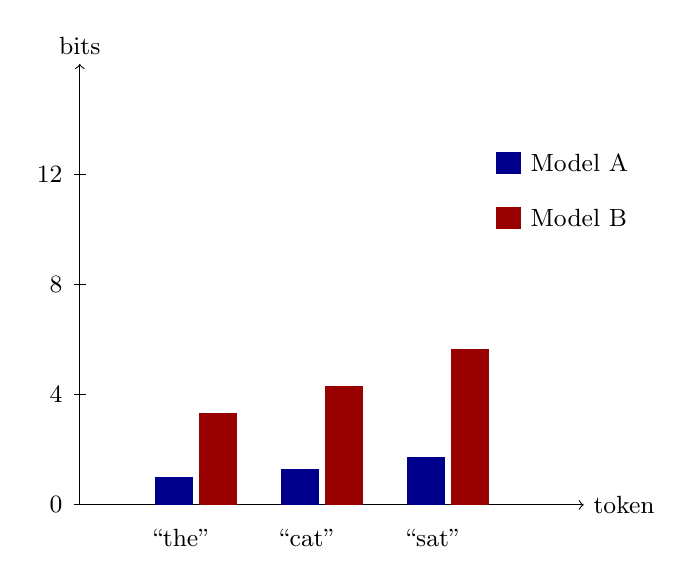
\begin{tikzpicture}[x=1.6cm, y=0.35cm]
  % axes
  \draw[->] (0,0) -- (4,0) node[right] {\small token};
  \draw[->] (0,0) -- (0,16) node[above] {\small bits};
  \foreach \y in {0,4,8,12} \draw (-0.05,\y) -- (0.05,\y) node[left,xshift=-5pt] {\small \y};
  % Model A bars (good): -log2(0.5, 0.4, 0.3) = 1.00, 1.32, 1.74
  \fill[blue!55!black] (0.6,0)  rectangle (0.9,1.00);
  \fill[blue!55!black] (1.6,0)  rectangle (1.9,1.32);
  \fill[blue!55!black] (2.6,0)  rectangle (2.9,1.74);
  % Model B bars (bad): -log2(0.1, 0.05, 0.02) = 3.32, 4.32, 5.64
  \fill[red!60!black]  (0.95,0) rectangle (1.25,3.32);
  \fill[red!60!black]  (1.95,0) rectangle (2.25,4.32);
  \fill[red!60!black]  (2.95,0) rectangle (3.25,5.64);
  % labels
  \node at (0.8,-1.2) {\small ``the''};
  \node at (1.8,-1.2) {\small ``cat''};
  \node at (2.8,-1.2) {\small ``sat''};
  % legend
  \fill[blue!55!black] (3.3,12) rectangle (3.5,12.8);
  \node[right] at (3.5,12.4) {\small Model A};
  \fill[red!60!black]  (3.3,10) rectangle (3.5,10.8);
  \node[right] at (3.5,10.4) {\small Model B};
\end{tikzpicture}
\caption{Per-token surprise $-\log_2 q(x_t\mid x_{<t})$ for the
sentence ``the cat sat'' under two toy models.  The total height is
the cross-entropy times $T$; the area difference is the KL
surcharge.  (\cref{act:python})}
\label{fig:surprise-bars}
\end{figure}


\begin{decisionbox}
\textbf{Three questions to ask an LLM vendor.}
\begin{enumerate}[leftmargin=*, itemsep=2pt]
  \item \emph{What is your held-out cross-entropy (or equivalently,
        perplexity) on a corpus we supply?}  This is the only
        vendor-agnostic compression score.
  \item \emph{Was the benchmark corpus demonstrably outside the
        training set?}  If not, the number is theatre.
  \item \emph{How much does a $0.1$-bit-per-token improvement cost in
        compute, and what does it buy at our deployment scale?}
        Use \cref{act:bytes} to translate bits into storage,
        bandwidth, or inference tokens.
\end{enumerate}
\end{decisionbox}

A worked numerical example separating the matched and mismatched
models on a $3$-token sequence is given in \cref{app:ce-worked};
\cref{act:python,act:bytes} above are the in-class shortcuts to the
same computation.

% =========================================================================
